\begin{song}{title=\predtitle\centering Kluziště \\\large Karel Plíhal \vspace*{-0.3cm}}  %% sem se napíše jméno songu a autor
\begin{centerjustified}
\nejvetsi

\sloka 
	^{C{\color{white}aaaa}}Strejček ^{Emi7/H}kovář ^{Ami7}chytil ^{C/G}kleště, 

	^{Fmaj7}uštíp' z ^{C}noční ^{\,\,\,Fmaj7\,\,G}oblohy
	
	jednu malou kapku deště, ta mu spadla pod nohy.
	
	Nejdřív ale chytil slinu, tak šáh' kamsi pro pivo,
	
	pak přitáhl kovadlinu a obrovský kladivo.

\refren
	Zatím ^{C}tři bílé ^{Emi7/H}vrány ^{Ami7}pěkně za ^{C/G}sebou
	
	kolem ^{Fmaj7}jdou, někam ^{C}jdou, do ^{D7}rytmu se ^{G}kývají,

	tyhle ^{C}tři bílé ^{Emi7/H}vrány ^{Ami7}pěkně za ^{C/G}sebou
	
	kolem ^{Fmaj7}jdou, někam ^{C}jdou, ^{Fmaj7}nedojdou, ^{C}nedojdou.

	\phantom{.}

\ssloka{\textbf{Mezihra}}


\sloka	
	Vydal z hrdla mocný pokřik ztichlým letním večerem,
	
	pak tu kapku všude rozstřík' jedním mocným úderem.
	
	Celej svět byl náhle v kapce a vysoko nad námi.
	
	Na obrovské mucholapce visí nebe s hvězdami.

\refren

\sloka
	Zpod víček mi vytrysk' pramen na zmačkané polštáře,
	
	kdosi mě vzal kolem ramen a políbil na tváře,
	
	kdesi v dálce rozmazaně strejda kovář odchází,
	
	do kalhot si čistí dlaně umazané od sazí. 

\refren

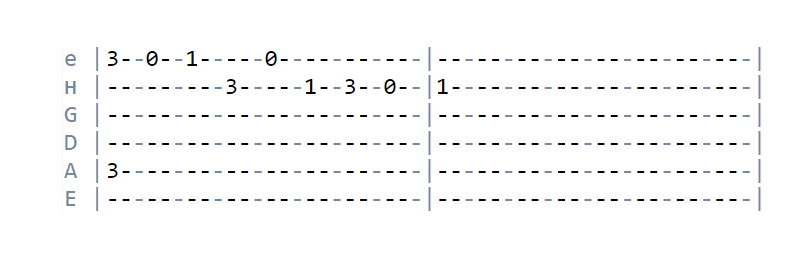
\includegraphics[scale=0.5]{../taby/kluziste.PNG}
\end{centerjustified}
\setcounter{Slokočet}{0}
\end{song}
